% Options for packages loaded elsewhere
% Options for packages loaded elsewhere
\PassOptionsToPackage{unicode}{hyperref}
\PassOptionsToPackage{hyphens}{url}
\PassOptionsToPackage{dvipsnames,svgnames,x11names}{xcolor}
%
\documentclass[
  letterpaper,
  DIV=11,
  numbers=noendperiod]{scrartcl}
\usepackage{xcolor}
\usepackage{amsmath,amssymb}
\setcounter{secnumdepth}{-\maxdimen} % remove section numbering
\usepackage{iftex}
\ifPDFTeX
  \usepackage[T1]{fontenc}
  \usepackage[utf8]{inputenc}
  \usepackage{textcomp} % provide euro and other symbols
\else % if luatex or xetex
  \usepackage{unicode-math} % this also loads fontspec
  \defaultfontfeatures{Scale=MatchLowercase}
  \defaultfontfeatures[\rmfamily]{Ligatures=TeX,Scale=1}
\fi
\usepackage{lmodern}
\ifPDFTeX\else
  % xetex/luatex font selection
\fi
% Use upquote if available, for straight quotes in verbatim environments
\IfFileExists{upquote.sty}{\usepackage{upquote}}{}
\IfFileExists{microtype.sty}{% use microtype if available
  \usepackage[]{microtype}
  \UseMicrotypeSet[protrusion]{basicmath} % disable protrusion for tt fonts
}{}
\makeatletter
\@ifundefined{KOMAClassName}{% if non-KOMA class
  \IfFileExists{parskip.sty}{%
    \usepackage{parskip}
  }{% else
    \setlength{\parindent}{0pt}
    \setlength{\parskip}{6pt plus 2pt minus 1pt}}
}{% if KOMA class
  \KOMAoptions{parskip=half}}
\makeatother
% Make \paragraph and \subparagraph free-standing
\makeatletter
\ifx\paragraph\undefined\else
  \let\oldparagraph\paragraph
  \renewcommand{\paragraph}{
    \@ifstar
      \xxxParagraphStar
      \xxxParagraphNoStar
  }
  \newcommand{\xxxParagraphStar}[1]{\oldparagraph*{#1}\mbox{}}
  \newcommand{\xxxParagraphNoStar}[1]{\oldparagraph{#1}\mbox{}}
\fi
\ifx\subparagraph\undefined\else
  \let\oldsubparagraph\subparagraph
  \renewcommand{\subparagraph}{
    \@ifstar
      \xxxSubParagraphStar
      \xxxSubParagraphNoStar
  }
  \newcommand{\xxxSubParagraphStar}[1]{\oldsubparagraph*{#1}\mbox{}}
  \newcommand{\xxxSubParagraphNoStar}[1]{\oldsubparagraph{#1}\mbox{}}
\fi
\makeatother

\usepackage{color}
\usepackage{fancyvrb}
\newcommand{\VerbBar}{|}
\newcommand{\VERB}{\Verb[commandchars=\\\{\}]}
\DefineVerbatimEnvironment{Highlighting}{Verbatim}{commandchars=\\\{\}}
% Add ',fontsize=\small' for more characters per line
\usepackage{framed}
\definecolor{shadecolor}{RGB}{241,243,245}
\newenvironment{Shaded}{\begin{snugshade}}{\end{snugshade}}
\newcommand{\AlertTok}[1]{\textcolor[rgb]{0.68,0.00,0.00}{#1}}
\newcommand{\AnnotationTok}[1]{\textcolor[rgb]{0.37,0.37,0.37}{#1}}
\newcommand{\AttributeTok}[1]{\textcolor[rgb]{0.40,0.45,0.13}{#1}}
\newcommand{\BaseNTok}[1]{\textcolor[rgb]{0.68,0.00,0.00}{#1}}
\newcommand{\BuiltInTok}[1]{\textcolor[rgb]{0.00,0.23,0.31}{#1}}
\newcommand{\CharTok}[1]{\textcolor[rgb]{0.13,0.47,0.30}{#1}}
\newcommand{\CommentTok}[1]{\textcolor[rgb]{0.37,0.37,0.37}{#1}}
\newcommand{\CommentVarTok}[1]{\textcolor[rgb]{0.37,0.37,0.37}{\textit{#1}}}
\newcommand{\ConstantTok}[1]{\textcolor[rgb]{0.56,0.35,0.01}{#1}}
\newcommand{\ControlFlowTok}[1]{\textcolor[rgb]{0.00,0.23,0.31}{\textbf{#1}}}
\newcommand{\DataTypeTok}[1]{\textcolor[rgb]{0.68,0.00,0.00}{#1}}
\newcommand{\DecValTok}[1]{\textcolor[rgb]{0.68,0.00,0.00}{#1}}
\newcommand{\DocumentationTok}[1]{\textcolor[rgb]{0.37,0.37,0.37}{\textit{#1}}}
\newcommand{\ErrorTok}[1]{\textcolor[rgb]{0.68,0.00,0.00}{#1}}
\newcommand{\ExtensionTok}[1]{\textcolor[rgb]{0.00,0.23,0.31}{#1}}
\newcommand{\FloatTok}[1]{\textcolor[rgb]{0.68,0.00,0.00}{#1}}
\newcommand{\FunctionTok}[1]{\textcolor[rgb]{0.28,0.35,0.67}{#1}}
\newcommand{\ImportTok}[1]{\textcolor[rgb]{0.00,0.46,0.62}{#1}}
\newcommand{\InformationTok}[1]{\textcolor[rgb]{0.37,0.37,0.37}{#1}}
\newcommand{\KeywordTok}[1]{\textcolor[rgb]{0.00,0.23,0.31}{\textbf{#1}}}
\newcommand{\NormalTok}[1]{\textcolor[rgb]{0.00,0.23,0.31}{#1}}
\newcommand{\OperatorTok}[1]{\textcolor[rgb]{0.37,0.37,0.37}{#1}}
\newcommand{\OtherTok}[1]{\textcolor[rgb]{0.00,0.23,0.31}{#1}}
\newcommand{\PreprocessorTok}[1]{\textcolor[rgb]{0.68,0.00,0.00}{#1}}
\newcommand{\RegionMarkerTok}[1]{\textcolor[rgb]{0.00,0.23,0.31}{#1}}
\newcommand{\SpecialCharTok}[1]{\textcolor[rgb]{0.37,0.37,0.37}{#1}}
\newcommand{\SpecialStringTok}[1]{\textcolor[rgb]{0.13,0.47,0.30}{#1}}
\newcommand{\StringTok}[1]{\textcolor[rgb]{0.13,0.47,0.30}{#1}}
\newcommand{\VariableTok}[1]{\textcolor[rgb]{0.07,0.07,0.07}{#1}}
\newcommand{\VerbatimStringTok}[1]{\textcolor[rgb]{0.13,0.47,0.30}{#1}}
\newcommand{\WarningTok}[1]{\textcolor[rgb]{0.37,0.37,0.37}{\textit{#1}}}

\usepackage{longtable,booktabs,array}
\usepackage{calc} % for calculating minipage widths
% Correct order of tables after \paragraph or \subparagraph
\usepackage{etoolbox}
\makeatletter
\patchcmd\longtable{\par}{\if@noskipsec\mbox{}\fi\par}{}{}
\makeatother
% Allow footnotes in longtable head/foot
\IfFileExists{footnotehyper.sty}{\usepackage{footnotehyper}}{\usepackage{footnote}}
\makesavenoteenv{longtable}
\usepackage{graphicx}
\makeatletter
\newsavebox\pandoc@box
\newcommand*\pandocbounded[1]{% scales image to fit in text height/width
  \sbox\pandoc@box{#1}%
  \Gscale@div\@tempa{\textheight}{\dimexpr\ht\pandoc@box+\dp\pandoc@box\relax}%
  \Gscale@div\@tempb{\linewidth}{\wd\pandoc@box}%
  \ifdim\@tempb\p@<\@tempa\p@\let\@tempa\@tempb\fi% select the smaller of both
  \ifdim\@tempa\p@<\p@\scalebox{\@tempa}{\usebox\pandoc@box}%
  \else\usebox{\pandoc@box}%
  \fi%
}
% Set default figure placement to htbp
\def\fps@figure{htbp}
\makeatother





\setlength{\emergencystretch}{3em} % prevent overfull lines

\providecommand{\tightlist}{%
  \setlength{\itemsep}{0pt}\setlength{\parskip}{0pt}}



 


\KOMAoption{captions}{tableheading}
\makeatletter
\@ifpackageloaded{caption}{}{\usepackage{caption}}
\AtBeginDocument{%
\ifdefined\contentsname
  \renewcommand*\contentsname{Table of contents}
\else
  \newcommand\contentsname{Table of contents}
\fi
\ifdefined\listfigurename
  \renewcommand*\listfigurename{List of Figures}
\else
  \newcommand\listfigurename{List of Figures}
\fi
\ifdefined\listtablename
  \renewcommand*\listtablename{List of Tables}
\else
  \newcommand\listtablename{List of Tables}
\fi
\ifdefined\figurename
  \renewcommand*\figurename{Figure}
\else
  \newcommand\figurename{Figure}
\fi
\ifdefined\tablename
  \renewcommand*\tablename{Table}
\else
  \newcommand\tablename{Table}
\fi
}
\@ifpackageloaded{float}{}{\usepackage{float}}
\floatstyle{ruled}
\@ifundefined{c@chapter}{\newfloat{codelisting}{h}{lop}}{\newfloat{codelisting}{h}{lop}[chapter]}
\floatname{codelisting}{Listing}
\newcommand*\listoflistings{\listof{codelisting}{List of Listings}}
\makeatother
\makeatletter
\makeatother
\makeatletter
\@ifpackageloaded{caption}{}{\usepackage{caption}}
\@ifpackageloaded{subcaption}{}{\usepackage{subcaption}}
\makeatother
\usepackage{bookmark}
\IfFileExists{xurl.sty}{\usepackage{xurl}}{} % add URL line breaks if available
\urlstyle{same}
\hypersetup{
  pdftitle={Python Fundamentals},
  colorlinks=true,
  linkcolor={blue},
  filecolor={Maroon},
  citecolor={Blue},
  urlcolor={Blue},
  pdfcreator={LaTeX via pandoc}}


\title{Python Fundamentals}
\author{}
\date{}
\begin{document}
\maketitle


\subsection{Objectives}\label{objectives}

\begin{itemize}
\tightlist
\item
  Assign values to variables.
\end{itemize}

This is a note that you can only see in presenter view

\subsection{Questions}\label{questions}

\begin{itemize}
\item
  What basic data types can I work with in Python?
\item
  How can I create a new variable in Python?
\item
  How do I use a function?
\item
  Can I change the value associated with a variable after I create it?
\item
  How can I get help while learning to program?
\end{itemize}

\subsection{Variables}\label{variables}

Any Python interpreter can be used as a calculator:

\begin{Shaded}
\begin{Highlighting}[]
\DecValTok{3} \OperatorTok{+} \DecValTok{5} \OperatorTok{*} \DecValTok{4}
\end{Highlighting}
\end{Shaded}

\begin{verbatim}
23
\end{verbatim}

This is great but not very interesting.

\subsection{Variable assignment}\label{variable-assignment}

To do anything useful with data, we need to assign its value to a
\emph{variable}. In Python, we can
\href{../learners/reference.md\#assign}{assign} a value to a
\href{../learners/reference.md\#variable}{variable}, using the equals
sign \texttt{=}. For example, we can track the weight of a patient who
weighs 60 kilograms by assigning the value \texttt{60} to a variable
\texttt{weight\_kg}:

\begin{Shaded}
\begin{Highlighting}[]
\NormalTok{weight\_kg }\OperatorTok{=} \DecValTok{60}
\BuiltInTok{print}\NormalTok{(weight\_kg)}
\end{Highlighting}
\end{Shaded}

\begin{verbatim}
60
\end{verbatim}

From now on, whenever we use \texttt{weight\_kg}, Python will substitute
the value we assigned to it. In layperson's terms, \textbf{a variable is
a name for a value}.

\subsection{Variable names In Python:}\label{variable-names-in-python}

variable names:

\begin{itemize}
\tightlist
\item
  can include letters, digits, and underscores
\item
  cannot start with a digit
\item
  are \href{../learners/reference.md\#case-sensitive}{case sensitive}.
\end{itemize}

This means that, for example:

\begin{itemize}
\tightlist
\item
  \texttt{weight0} is a valid variable name, whereas \texttt{0weight} is
  not
\item
  \texttt{weight} and \texttt{Weight} are different variables
\end{itemize}

\subsection{Types of data}\label{types-of-data}

Python knows various types of data. Three common ones are:

\begin{itemize}
\tightlist
\item
  integer numbers
\item
  floating point numbers, and
\item
  strings.
\end{itemize}

In the example above, variable \texttt{weight\_kg} has an integer value
of \texttt{60}.

\begin{center}\rule{0.5\linewidth}{0.5pt}\end{center}

If we want to more precisely track the weight of our patient, we can use
a floating point value by executing:

\begin{Shaded}
\begin{Highlighting}[]
\NormalTok{weight\_kg }\OperatorTok{=} \FloatTok{60.3}
\BuiltInTok{print}\NormalTok{(weight\_kg)}
\end{Highlighting}
\end{Shaded}

\begin{verbatim}
60.3
\end{verbatim}

\begin{center}\rule{0.5\linewidth}{0.5pt}\end{center}

To create a string, we add single or double quotes around some text. To
identify and track a patient throughout our study, we can assign each
person a unique identifier by storing it in a string:

\begin{Shaded}
\begin{Highlighting}[]
\NormalTok{patient\_id }\OperatorTok{=} \StringTok{\textquotesingle{}001\textquotesingle{}}
\BuiltInTok{print}\NormalTok{(patient\_id)}
\end{Highlighting}
\end{Shaded}

\begin{verbatim}
001
\end{verbatim}

\subsection{Using Variables in Python}\label{using-variables-in-python}

Once we have data stored with variable names, we can make use of it in
calculations. We may want to store our patient's weight in pounds as
well as kilograms:

\begin{Shaded}
\begin{Highlighting}[]
\NormalTok{weight\_lb }\OperatorTok{=} \FloatTok{2.2} \OperatorTok{*}\NormalTok{ weight\_kg}
\BuiltInTok{print}\NormalTok{(weight\_lb)}
\end{Highlighting}
\end{Shaded}

\begin{verbatim}
132.66
\end{verbatim}

We might decide to add a prefix to our patient identifier:

\begin{Shaded}
\begin{Highlighting}[]
\NormalTok{patient\_id }\OperatorTok{=} \StringTok{\textquotesingle{}inflam\_\textquotesingle{}} \OperatorTok{+}\NormalTok{ patient\_id}
\BuiltInTok{print}\NormalTok{(patient\_id)}
\end{Highlighting}
\end{Shaded}

\begin{verbatim}
inflam_001
\end{verbatim}

\subsection{Built-in Python functions}\label{built-in-python-functions}

To carry out common tasks with data and variables in Python, the
language provides us with several built-in
\href{../learners/reference.md\#function}{functions}. To display
information to the screen, we use the \texttt{print} function:

\begin{Shaded}
\begin{Highlighting}[]
\BuiltInTok{print}\NormalTok{(weight\_lb)}
\end{Highlighting}
\end{Shaded}

\begin{verbatim}
132.66
\end{verbatim}

\begin{Shaded}
\begin{Highlighting}[]
\BuiltInTok{print}\NormalTok{(patient\_id)}
\end{Highlighting}
\end{Shaded}

\begin{verbatim}
inflam_001
\end{verbatim}

\subsection{Parentheses}\label{parentheses}

When we want to make use of a function, referred to as calling the
function, we follow its name by parentheses. The parentheses are
important: if you leave them off, the function doesn't actually run!
Sometimes you will include values or variables inside the parentheses
for the function to use. In the case of \texttt{print}, we use the
parentheses to tell the function what value we want to display. We will
learn more about how functions work and how to create our own in later
episodes.

\subsection{Combining outputs using
``print''}\label{combining-outputs-using-print}

We can display multiple things at once using only one \texttt{print}
call:

\begin{Shaded}
\begin{Highlighting}[]
\BuiltInTok{print}\NormalTok{(patient\_id, }\StringTok{\textquotesingle{}weight in kilograms:\textquotesingle{}}\NormalTok{, weight\_kg)}
\end{Highlighting}
\end{Shaded}

\begin{verbatim}
inflam_001 weight in kilograms: 60.3
\end{verbatim}

\begin{Shaded}
\begin{Highlighting}[]
\FunctionTok{print}\NormalTok{(}\StringTok{"hello world"}\NormalTok{)}
\end{Highlighting}
\end{Shaded}

\begin{verbatim}
[1] "hello world"
\end{verbatim}

\subsection{Nested Functions}\label{nested-functions}

We can also call a function inside of another
\href{../learners/reference.md\#function-call}{function call}. For
example, Python has a built-in function called \texttt{type} that tells
you a value's data type:

\begin{Shaded}
\begin{Highlighting}[]
\BuiltInTok{print}\NormalTok{(}\BuiltInTok{type}\NormalTok{(}\FloatTok{60.3}\NormalTok{))}
\end{Highlighting}
\end{Shaded}

\begin{verbatim}
<class 'float'>
\end{verbatim}

\begin{Shaded}
\begin{Highlighting}[]
\BuiltInTok{print}\NormalTok{(}\BuiltInTok{type}\NormalTok{(patient\_id))}
\end{Highlighting}
\end{Shaded}

\begin{verbatim}
<class 'str'>
\end{verbatim}

\subsection{Nested Print}\label{nested-print}

Moreover, we can do arithmetic with variables right inside the
\texttt{print} function:

\begin{Shaded}
\begin{Highlighting}[]
\BuiltInTok{print}\NormalTok{(}\StringTok{\textquotesingle{}weight in pounds:\textquotesingle{}}\NormalTok{, }\FloatTok{2.2} \OperatorTok{*}\NormalTok{ weight\_kg)}
\end{Highlighting}
\end{Shaded}

\begin{verbatim}
weight in pounds: 132.66
\end{verbatim}

Note: The above command, however, did not change the value of
\texttt{weight\_kg}:

\begin{Shaded}
\begin{Highlighting}[]
\BuiltInTok{print}\NormalTok{(weight\_kg)}
\end{Highlighting}
\end{Shaded}

\begin{verbatim}
60.3
\end{verbatim}

\subsection{Updating variables}\label{updating-variables}

To change the value of the \texttt{weight\_kg} variable, we have to
\textbf{assign} \texttt{weight\_kg} a new value using the equals
\texttt{=} sign:

\begin{Shaded}
\begin{Highlighting}[]
\NormalTok{weight\_kg }\OperatorTok{=} \FloatTok{65.0}
\BuiltInTok{print}\NormalTok{(}\StringTok{\textquotesingle{}weight in kilograms is now:\textquotesingle{}}\NormalTok{, weight\_kg)}
\end{Highlighting}
\end{Shaded}

\begin{verbatim}
weight in kilograms is now: 65.0
\end{verbatim}

\subsection{Getting Help}\label{getting-help}

Use the built-in function \texttt{help} to get help for a function.
Every built-in function has extensive
\href{https://docs.python.org/3/library/index.html}{documentation that
can also be found online}.

\subsection{Help Example}\label{help-example}

\begin{Shaded}
\begin{Highlighting}[]
\BuiltInTok{help}\NormalTok{(}\BuiltInTok{print}\NormalTok{)}
\end{Highlighting}
\end{Shaded}

\begin{verbatim}
Help on built-in function print in module builtins:

print(...)
    print(value, ..., sep=' ', end='\n', file=sys.stdout, flush=False)
    
    Prints the values to a stream, or to sys.stdout by default.
    Optional keyword arguments:
    file:  a file-like object (stream); defaults to the current sys.stdout.
    sep:   string inserted between values, default a space.
    end:   string appended after the last value, default a newline.
    flush: whether to forcibly flush the stream.
\end{verbatim}

This help message (the function's ``docstring'') includes a usage
statement, a list of parameters accepted by the function, and their
default values if they have them.

\subsection{Error messages}\label{error-messages}

It is normal to encounter error messages while programming, whether you
are learning for the first time or have been programming for many years.
\href{./09-errors.md}{We will discuss error messages in more detail
later}. For now, let's explore how people use them to get more help when
they are stuck with their Python code.

\subsection{Task 1}\label{task-1}

Search the internet: paste the last line of your error message or the
word ``python'' and a short description of what you want to do into your
favourite search engine and you will usually find several examples where
other people have encountered the same problem and came looking for
help.

\subsection{Hints}\label{hints}

\href{https://stackoverflow.com/questions}{StackOverflow} can be
particularly helpful for this: answers to questions are presented as a
ranked thread ordered according to how useful other users found them to
be.

\textbf{Take care:} copying and pasting code written by somebody else is
risky unless you understand exactly what it is doing!

\subsection{Alternative approach}\label{alternative-approach}

Ask somebody ``in the real world''.

If you have a colleague or friend with more expertise in Python than you
have, show them the problem you are having and ask them for help.

\href{./11-debugging.md}{We will discuss more debugging strategies in
greater depth later in the lesson}.

\subsection{Variables as Sticky Notes}\label{variables-as-sticky-notes}

A variable in Python is analogous to a sticky note with a name written
on it: assigning a value to a variable is like putting that sticky note
on a particular value.

\pandocbounded{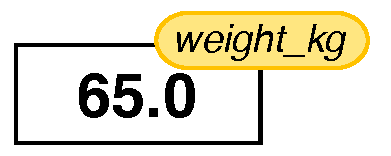
\includegraphics[keepaspectratio]{01-intro_files/mediabag/fig/python-sticky-note-variables-01.pdf}}

\begin{center}\rule{0.5\linewidth}{0.5pt}\end{center}

Using this analogy, we can investigate how assigning a value to one
variable does \textbf{not} change values of other, seemingly related,
variables. For example, let's store the subject's weight in pounds in
its own variable:

\begin{Shaded}
\begin{Highlighting}[]
\CommentTok{\# There are 2.2 pounds per kilogram}
\NormalTok{weight\_lb }\OperatorTok{=} \FloatTok{2.2} \OperatorTok{*}\NormalTok{ weight\_kg}
\BuiltInTok{print}\NormalTok{(}\StringTok{\textquotesingle{}weight in kilograms:\textquotesingle{}}\NormalTok{, weight\_kg, }\StringTok{\textquotesingle{}and in pounds:\textquotesingle{}}\NormalTok{, weight\_lb)}
\end{Highlighting}
\end{Shaded}

\begin{verbatim}
weight in kilograms: 65.0 and in pounds: 143.0
\end{verbatim}

\subsection{Commenting}\label{commenting}

Everything in a line of code following the `\#' symbol is a
\href{../learners/reference.md\#comment}{comment} that is ignored by
Python. Comments allow programmers to leave explanatory notes for other
programmers or their future selves.

\subsection{Variable Dependancies}\label{variable-dependancies}

\pandocbounded{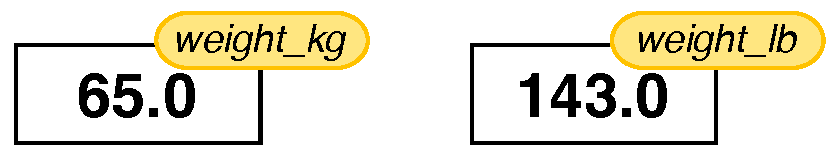
\includegraphics[keepaspectratio]{01-intro_files/mediabag/fig/python-sticky-note-variables-02.pdf}}

Similar to above, the expression \texttt{2.2\ *\ weight\_kg} is
evaluated to \texttt{143.0}, and then this value is assigned to the
variable \texttt{weight\_lb} (i.e.~the sticky note \texttt{weight\_lb}
is placed on \texttt{143.0}). At this point, each variable is ``stuck''
to completely distinct and unrelated values.

\begin{center}\rule{0.5\linewidth}{0.5pt}\end{center}

Let's now change \texttt{weight\_kg}:

\begin{Shaded}
\begin{Highlighting}[]
\NormalTok{weight\_kg }\OperatorTok{=} \FloatTok{100.0}
\BuiltInTok{print}\NormalTok{(}\StringTok{\textquotesingle{}weight in kilograms is now:\textquotesingle{}}\NormalTok{, weight\_kg, }\StringTok{\textquotesingle{}and weight in pounds is still:\textquotesingle{}}\NormalTok{, weight\_lb)}
\end{Highlighting}
\end{Shaded}

\begin{verbatim}
weight in kilograms is now: 100.0 and weight in pounds is still: 143.0
\end{verbatim}

\pandocbounded{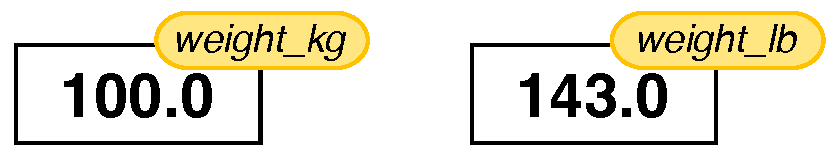
\includegraphics[keepaspectratio]{01-intro_files/mediabag/fig/python-sticky-note-variables-03.pdf}}

Since \texttt{weight\_lb} doesn't ``remember'' where its value comes
from, it is not updated when we change \texttt{weight\_kg}.

\subsection{Task 2: Check Your
Understanding}\label{task-2-check-your-understanding}

\subsubsection{Question:}

What values do the variables \texttt{mass} and \texttt{age} have after
each of the following statements? Test your answer by executing the
lines.

\begin{Shaded}
\begin{Highlighting}[]
\NormalTok{mass }\OperatorTok{=} \FloatTok{47.5}
\NormalTok{age }\OperatorTok{=} \DecValTok{122}
\NormalTok{mass }\OperatorTok{=}\NormalTok{ mass }\OperatorTok{*} \FloatTok{2.0}
\NormalTok{age }\OperatorTok{=}\NormalTok{ age }\OperatorTok{{-}} \DecValTok{20}
\end{Highlighting}
\end{Shaded}

\subsubsection{Solution}

\begin{Shaded}
\begin{Highlighting}[]
\NormalTok{mass }\OperatorTok{=} \FloatTok{47.5}
\BuiltInTok{print}\NormalTok{(mass)}
\end{Highlighting}
\end{Shaded}

\begin{verbatim}
47.5
\end{verbatim}

\begin{Shaded}
\begin{Highlighting}[]
\NormalTok{age }\OperatorTok{=} \DecValTok{122}
\BuiltInTok{print}\NormalTok{(age)}
\end{Highlighting}
\end{Shaded}

\begin{verbatim}
122
\end{verbatim}

\begin{Shaded}
\begin{Highlighting}[]
\NormalTok{mass }\OperatorTok{=}\NormalTok{ mass }\OperatorTok{*} \FloatTok{2.0}
\BuiltInTok{print}\NormalTok{(mass)}
\end{Highlighting}
\end{Shaded}

\begin{verbatim}
95.0
\end{verbatim}

\begin{Shaded}
\begin{Highlighting}[]
\NormalTok{age }\OperatorTok{=}\NormalTok{ age }\OperatorTok{{-}} \DecValTok{20}
\BuiltInTok{print}\NormalTok{(age)}
\end{Highlighting}
\end{Shaded}

\begin{verbatim}
102
\end{verbatim}

\subsection{Task 3: Sorting Out
References}\label{task-3-sorting-out-references}

\subsubsection{Question:}

Python allows you to assign multiple values to multiple variables in one
line by separating the variables and values with commas. What does the
following program print out?

\begin{Shaded}
\begin{Highlighting}[]
\NormalTok{first, second }\OperatorTok{=} \StringTok{\textquotesingle{}Grace\textquotesingle{}}\NormalTok{, }\StringTok{\textquotesingle{}Hopper\textquotesingle{}}
\NormalTok{third, fourth }\OperatorTok{=}\NormalTok{ second, first}
\end{Highlighting}
\end{Shaded}

\subsubsection{Solution}

\begin{Shaded}
\begin{Highlighting}[]
\BuiltInTok{print}\NormalTok{(third, fourth)}
\end{Highlighting}
\end{Shaded}

\begin{verbatim}
Hopper Grace
\end{verbatim}

\subsection{Task 4: Seeing Data Types}\label{task-4-seeing-data-types}

\subsubsection{Question:}

What are the data types of the following variables?

\begin{Shaded}
\begin{Highlighting}[]
\NormalTok{planet }\OperatorTok{=} \StringTok{\textquotesingle{}Earth\textquotesingle{}}
\NormalTok{apples }\OperatorTok{=} \DecValTok{5}
\NormalTok{distance }\OperatorTok{=} \FloatTok{10.5}
\end{Highlighting}
\end{Shaded}

\subsubsection{Solution}

\begin{Shaded}
\begin{Highlighting}[]
\BuiltInTok{print}\NormalTok{(}\BuiltInTok{type}\NormalTok{(planet))}
\end{Highlighting}
\end{Shaded}

\begin{verbatim}
<class 'str'>
\end{verbatim}

\begin{Shaded}
\begin{Highlighting}[]
\BuiltInTok{print}\NormalTok{(}\BuiltInTok{type}\NormalTok{(apples))}
\end{Highlighting}
\end{Shaded}

\begin{verbatim}
<class 'int'>
\end{verbatim}

\begin{Shaded}
\begin{Highlighting}[]
\BuiltInTok{print}\NormalTok{(}\BuiltInTok{type}\NormalTok{(distance))}
\end{Highlighting}
\end{Shaded}

\begin{verbatim}
<class 'float'>
\end{verbatim}

\subsection{keypoints}\label{keypoints}

\begin{itemize}
\tightlist
\item
  Basic data types in Python include integers, strings, and
  floating-point numbers.
\item
  Variables are created on demand whenever a value is assigned to them.
\item
  Built-in functions are always available to use.
\item
  Error messages provide information about what has gone wrong with your
  program and where.
\end{itemize}

\subsection{hints}\label{hints-1}

\begin{itemize}
\tightlist
\item
  Use \texttt{variable\ =\ value} to assign a value to a variable in
  order to record it in memory.
\item
  Use \texttt{print(something)} to display the value of
  \texttt{something}.
\item
  Use \texttt{\#\ some\ kind\ of\ explanation} to add comments to
  programs.
\item
  Use \texttt{help(thing)} to view help for something.
\end{itemize}




\end{document}
